
\begin{figure}[t!]
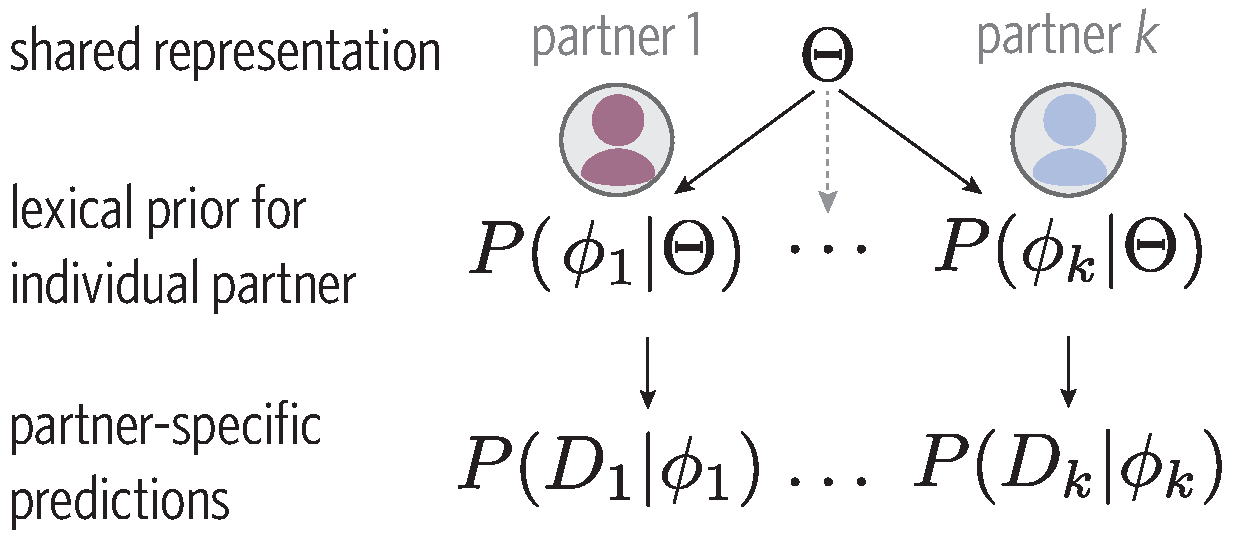
\includegraphics[scale=0.4]{./figures/task1_model.pdf}
\caption{Schematic of hierarchical Bayesian model.}
\label{fig:model_schematic}
\end{figure}

%\subsection{Hierarchical inference: generalizing to new partners}

In this section, we provide an explicit computational account of the cognitive mechanisms supporting the balance between community-level stability and partner-specific flexibility.
Our model is based on three basic principles: 

\begin{enumerate}
\item \emph{lexical uncertainty}, the idea that beliefs about the underlying conventions used by other agents are represented and updated probabilistically \cite{bergen_pragmatic_2016}
\item \emph{pragmatic reasoning}, the idea that agents expect other agents to use language in a cooperative manner, and do so themselves  \cite{GoodmanFrank16_RSATiCS}
\item \emph{inductive learning}, the idea that agents expect some abstract structure to be shared by their entire community, even by individuals they have never met \cite{}
\end{enumerate}

We formalize these principles in a hierarchical Bayesian model.
In a hierarchical model, the agent's uncertainty is represented by a multi-level prior. 
At the highest level of the hierarchy is \emph{community-level} uncertainty $P(\Theta)$, where $\Theta$ represents an abstract ``overhypothesis" about the overall distribution of possible partners. 
$\Theta$ then parameterizes the agent's \emph{partner-specific} uncertainty $P(\phi_{k} | \Theta)$, where $\phi_k$ represents the specific system of meaning used by partner $k$ (see Fig. \ref{fig:model_schematic}). 

Given observations $D_k$ from interactions with partner $k$, the agent updates their beliefs about the latent system of meaning using Bayes rule:
\begin{equation}
\begin{array}{rcl}
\label{eq:joint_inference}
P(\phi_k, \Theta | D_k)  & \propto &  P(D_k | \phi_k, \Theta) P(\phi_k, \Theta) \\
                           & =   & P(D_k | \phi_k) P(\phi_k | \Theta) P(\Theta)
\end{array}
\end{equation}
This joint inference decomposes the learning problem into two terms, a prior term $P(\phi_k | \Theta)P(\Theta)$ and a likelihood term $P(D_k | \phi_k)$.
The prior captures the idea that different partners may share aspects of meaning in common.
In the absence of strong evidence that partner-specific language use departs from this common structure, the agent ought to regularize toward background knowledge of the population's conventions.
The likelihood represents predictions about how a partner using a particular system of meaning will use language in context.

This joint posterior over meanings has two consequences for convention formation.
First, it allows agents to maintain partner-specific expectations $\phi_k$ by marginalizing over community-level uncertainty:
\begin{equation}
P(\phi_k | D_k) = \int_{\Theta}P(D_k | \phi_k) P(\phi_k | \Theta) P(\Theta)  d\Theta
\end{equation}
Second, the hierarchical structure provides an inductive pathway for data to inform beliefs about community-wide conventions.
Agents update their beliefs about $\Theta$ by marginalizing over data accumulated from different partners:
\begin{equation}
P(\Theta | D) = P(\Theta) \int_{\phi} P(D_k | \phi_k) P(\phi_k | \Theta) d\phi
\end{equation}
where $D = \bigcup_{k=1}^N D_k$, $\phi = \phi_1 \times \dots \times \phi_N$, and $N$ is the number of partners previous encountered. 
After multiple partners are inferred to have a similar system of meaning, beliefs about $\Theta$ shift to represent this abstracted knowledge: it becomes more likely that a novel partner will share it as well.
This transfer is sometimes referred to as ``sharing of strength'' or ``partial pooling'' because pooled data is smoothly integrated with domain-specific knowledge.

The principle of pragmatic reasoning enters our model at two distinct phases.
First, when an agent is inferring their partner's latent representation of meaning from their observable behavior (Eq. \ref{eq:joint_inference}), we assume that the likelihood reflects Gricean principles.
In other words, the agent assumes their partner is using language in a cooperative manner.
Second, agents do not only make passive inferences from data, they actually \emph{use language} in interaction, given their current beliefs.
We assume that this generative behavior is also guided by Gricean principles.

\todo[inline]{Swap in description of RSA from cogsci paper...}
In both cases, we formalize Gricean principles using the Rational Speech Act model, which has successfully accounted for a wide range of classic pragmatic as a consequence of basic mechanisms of social reasoning. 
A pragmatic speaker, denoted by $S_1$, attempts to be informative in context while a pragmatic listener, denoted by $L_1$, inverts an internal model of the speaker to infer the intended target. 
The chain of recursive social reasoning grounds out in a \emph{literal listener} $L_0$, which directly soft-maximizes its lexicon, $\mathcal{L}^t(w,o)$, to interpret a given utterance. 
This model can be formally specified as follows:
$$
\begin{array}{rcl}
L_0(o_i | w, \mathcal{L}^t) &\propto  & \exp\{\mathcal{L}^t(w,o_i)\} \\
S_1(w | o_i, \mathcal{L}^t) &\propto & \exp\{\ln L_0(o_i | w, \mathcal{L}^t)\} \\
L_1(o_i | w, \mathcal{L}^t) &\propto  & S_1(w | o_i, \mathcal{L}^t) P(o_i) 
\end{array}
$$
% MF: adjusted this for better vertical spacing wrt adjacent paragraphs
where $o_i$ is a chosen object and $w$ an uttered word.

\todo[inline]{Describe some more specific mechanisms that are shared across the simulations.
(1) memory discounting, (2) lexicon prior (simplicity + space of hypotheses for each word?), (3) how we ensure normalization is well-defined w/ null utterance (i.e. handling case where a word doesn't apply to any of the objects),}